\section{Architecture Integration}

\subsection{Model Support}

\begin{table}[H]
\centering
\small
\begin{tabular}{lllll}
\toprule
\textbf{Model} & \textbf{Attention path} & \textbf{Nested?} & \textbf{RoPE?} & \textbf{GQA?} \\
\midrule
DistilBERT & \texttt{layer[i].attention} & No & No & No \\
RoBERTa & \texttt{layer[i].attention.self} & Yes & No & No \\
GPT-2 & \texttt{h[i].attn} & No & No & No \\
Qwen3.5 & \texttt{layers[i].self\_attn} & No & Yes & Yes \\
\bottomrule
\end{tabular}
\end{table}

\subsection{Weight Extraction}

Handles four patterns (UniversalAdapter first, then fallbacks).

\subsubsection{GPT-2 Conv1D}

\begin{lstlisting}
c\_w = src.c\_attn.weight
if c\_w.shape[0] \textless{} c\_w.shape[1]: c\_w = c\_w.t()
q\_w, k\_w, v\_w = c\_w.chunk(3, dim=0)
o\_w = src.c\_proj.weight.t()
\end{lstlisting}

\subsubsection{RoBERTa Nested}

\begin{lstlisting}
s = src.self
q\_w = s.query.weight
k\_w = s.key.weight
v\_w = s.value.weight
o\_w = src.output.dense.weight
\end{lstlisting}

\subsubsection{Flat Modules}

\begin{lstlisting}
q\_w = src.q\_lin.weight  # or q\_proj or query
k\_w = src.k\_lin.weight
v\_w = src.v\_lin.weight
o\_w = src.out\_lin.weight
\end{lstlisting}

\subsection{Soft Fallback}

On missing weights, we log a warning and keep Kaiming defaults.

\subsection{Second Q-K Pair}

$W_{Q_2}, W_{K_2}$ are Kaiming-initialized and never copied -- the parent 
model has no analogue.

\subsection{The Bottleneck}

$W_\text{down}, W_\text{up}$ are randomly initialized (default PyTorch 
init) and trained. They do not need pretrained weights because they 
represent an \textbf{arbitrary} concept space.

\textbf{Optional:} Future work could initialize from PCA of activations (see 
Appendix D).

\subsection{Injection Algorithm}

\textbf{Algorithm 2:} Inject JambaInfo into a layer
\begin{lstlisting}
Input:  layer, config
Output: layer with attention replaced

1: src $\leftarrow$ extract\_attention(layer)
2: if src is None: return None
3: try:
4:     new $\leftarrow$ JambaInfoBlock(config, old\_attn=src)
5:     replace(layer, new)
6:     return new
7: except Exception:
8:     log\_error
9:     return None
\end{lstlisting}

\subsection{Nested Encoder Handling}

For RoBERTa, \texttt{is\_nested\_encoder = True}. The forward pass returns raw 
context, and the outer \texttt{output.dense} applies the projection.

\subsection{Causality}

Both attention maps and the SSM are causally masked for decoders.

\subsection{Cross-Attention}

Not supported. JambaInfo is encoder-only or decoder-only.

\subsection{Registry}

\begin{lstlisting}
@ATTENTION\_REGISTRY.register("jamba\_info")
class JambaInfoBlock(BaseAttention):
    ...

@ATTENTION\_REGISTRY.register("jamba\_info\_inject")
def inject\_jamba\_info(...):
    ...
\end{lstlisting}
\begin{lstlisting}

---
\end{lstlisting}

\begin{figure}[H]
\centering
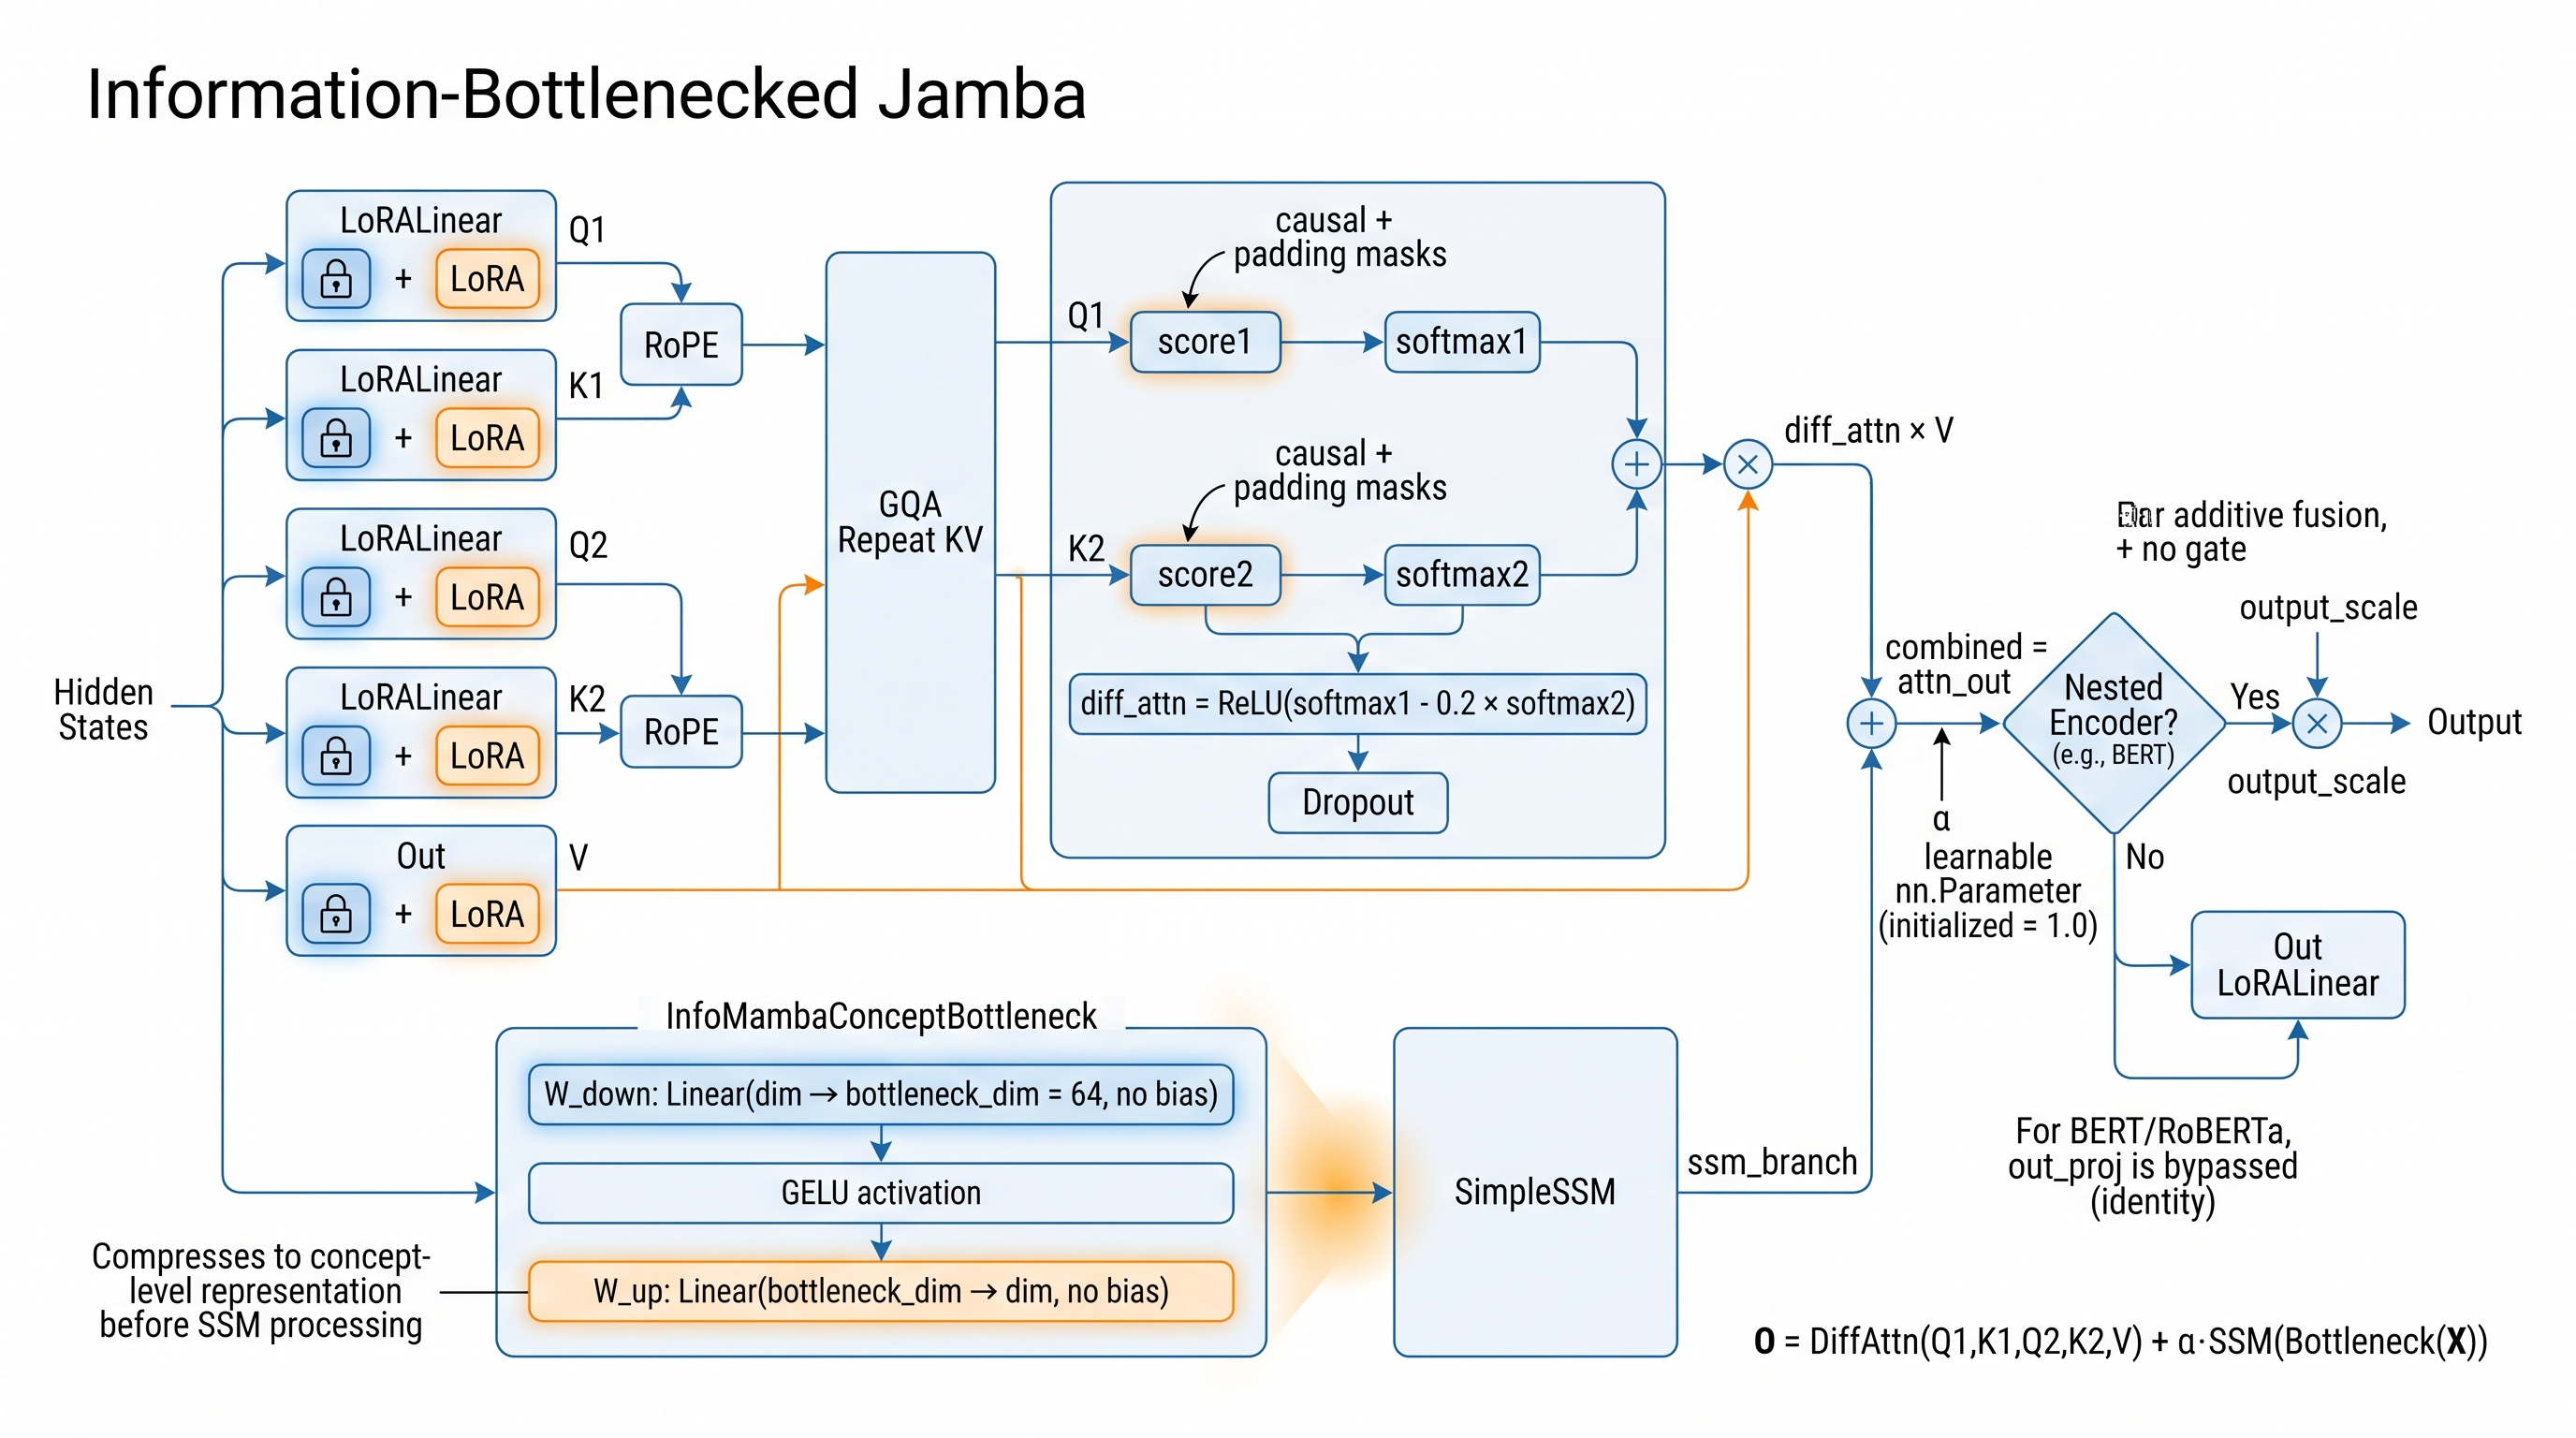
\includegraphics[width=\linewidth]{figures/architecture.jpeg}
\caption{High-level architectural diagram of jamba\_info.}
\label{fig:arch_jamba-info}
\end{figure}

